
\section{The Anykernel and Rump Kernels}
\label{chap:concept}

As a primer for the technical discussion in this document, we
consider the elements that make up a modern Unix-style operating system
kernel.  The following is not the only way to make a classification,
but it is the most relevant one for our coming discussion.

The \textit{CPU specific code} is on the bottom layer of the
OS.  This code takes care of low level bootstrap and provides an
abstract interface to the hardware.  In most, if not all, modern
general purpose operating systems the CPU architecture is abstracted away
from the bulk of the kernel and only the lowest layers have knowledge
of it.  To put the previous statement into terms which are used in our
later discussions, the interfaces provided by the CPU specific code are
the hypercall interfaces that the OS runs on.  In the NetBSD
kernel these functions are usually prefixed with ``\texttt{cpu}''.

The \textit{virtual memory subsystem} manages the virtual address space of
the kernel and processes.  Virtual memory management includes defining what
happens when a memory address is accessed.  Examples include
normal read/write access to the memory, flagging a segmentation violation,
or a file being read from the file system.

The \textit{process execution subsystem} understands the formats that
executable binaries use and knows how to create a new process when an
executable is run.

The \textit{scheduling code} includes a method and policy to define what
code a CPU is executing.  The currently executing thread can be switched
either when the scheduler decides it has run too long, or when the thread
itself makes a system call which requires waiting for a condition to
become true before execution can be resumed.  When a thread is switched,
the scheduler calls the CPU specific code to save the machine context of
the current thread and load the context of the new thread.  In NetBSD,
both user processes and the kernel are preemptively scheduled, meaning
the scheduler can decide to unschedule the currently executing thread
and schedule a new one.

\textit{Atomic operations} enable modifying memory atomically and
avoid race conditions in for example a read-modify-write cycle.
For uniprocessor architectures, kernel atomic operations are a matter of
disabling interrupts and preemption for the duration of the operation.
Multiprocessor architectures provide machine instructions for atomic
operations.  The operating system's role with atomic operations is mapping
function interfaces to the way atomic operations are implemented on that
particular machine architecture.

\textit{Synchronization routines} such as mutexes and condition
variables build upon atomic operations and interface with the scheduler.
For example, if locking a mutex is attempted, the condition for it being
free is atomically tested and set.  If a sleep mutex was already locked,
the currently executing thread interfaces with the scheduling code to
arrange for itself to be put to sleep until the mutex is released.

Various \textit{support interfaces} such CPU cross-call, time-related
routines, kernel linkers, etc. provide a basis on which to build drivers.

\textit{Resource management} includes general purpose memory
allocation, a pool and slab~\cite{bonwick:slab} allocator, file
descriptors, PID namespace, vmem/extent resource allocators etc.
Notably, in addition to generic resources such as memory,
there are more specific resources to manage.  Examples
of more specific resources include vnodes~\cite{kleiman:vnodes} for file
systems and mbufs~\cite{stevens:tcpip2} for the TCP/IP stack.

\textit{Drivers} interact with external objects such as file
system images, hardware, the network, etc.  After a fashion, it
can be said they accomplish all the useful work an operating system
does.  It needs to be remembered, though, that they operate
by building on top of the entities mentioned earlier in this section.
Drivers are what we are ultimately interested in utilizing, but to
make them available we must deal with everything they depend on.
Being able to reuse drivers means we have to provide semantically
equivalent implementations of the support routines that the drivers use.
The straightforward way is to run the entire kernel, but it not always
the optimal approach, as we will demonstrate throughout this book.

\subsection{An Ultralightweight Virtual Kernel for Drivers}
\label{sect:conceptintro}

Virtualization of the entire operating system can done either by
modifying the operating system kernel by means of paravirtualization
(\eg User-Mode Linux~\cite{dike:uml} or Xen~\cite{barham:xen}) or by virtualizing at the
hardware layer so than an unmodified operating system can be run
(by using \eg QEMU~\cite{bellard:qemu}).  From the perspective of
the host, virtualization provides both multiplicity and isolation
of the monolithic kernel, and can be seen as a possible solution
for our security and testing challenges from Section~\ref{sect:challenge}.
Using a fully virtualized OS as an application library is less
straightforward, but can be done by bootstrapping a guest instance
of an operating system and communicating with the guest's kernel
through an application running on the guest.  For example,
libguestfs~\cite{libguestfs} uses this approach to access file
system images safely.

Full OS virtualization is a heavyweight operation.  For
instance, several seconds of bootstrap delay for a fully virtualized
OS~\cite{jiang:soda} is too long if we wish to use virtualized
kernel instances as application libraries --- humans perceive delays
of over 100ms~\cite{miller:100ms}.  While it may be possible to
amortize the bootstrap delay over several invocations, managing
cached instances adds complexity to the applications, especially
if multiple different users want to use ones for multiple different
purposes.  Furthermore, a full OS consumes more machine resources,
such as memory and storage and CPU, than is necessary for kernel
driver virtualization.  The increased resource requirement is because
a full OS provides the entire application environment, which from our
perspective is overhead.

Virtualization via containers~\cite{phk:jails} provides better
performance than
paravirtualization~\cite{soltesz:containers,wang:overhead}.
However, containers do not address our motivating problems.
With containers, the host kernel is directly used for the purposes
of all guests.  In other words, kernel drivers are run in a single
domain within the host.  There is no isolation between kernel
drivers for different guests and a single error in one of them can
bring all of the guests and the host down.  The lack of isolation is due
to the use case that containers are targeted at: they provide a virtual
application environment instead of a virtual kernel environment.

We wish to investigate a lightweight solution to maximize the
performance and simplicity in our use cases.  In other words, we
believe in an approach which requires only the essential
functionality necessary for solving a
problem~\cite{lampson:bestpaperever}.

\subsubsection{Partial Virtualization and Relegation}

A key observation in our lightweight approach is that part of the
supporting functionality required by drivers is readily provided
by the system hosting our virtualized driver environment.  For
example, drivers need a memory address space to execute in; we use
the one that the host provides instead of simulating a second one
on top of it.  Likewise, we directly use the host's threading and
scheduling facilities in our virtual kernel instead of having the
host schedule a virtual kernel with its own layer of scheduling.
Relegating support functionality to the host avoids adding a layer
of indirection and overhead.  It is also the reason why we call
our virtualized kernel instance a \textit{rump kernel}: it virtualizes
only a part of the original.  In terms of taxonomy, we classify a
rump kernel as partial paravirtualization.

Drivers in a rump kernel remain unmodified over the original ones.
A large part of the support routines remain unmodified as well.
Only in places where support is relegated to the host, do we require
specifically written glue code.  We use the term \textit{anykernel} to describe
 a kernel code base with the property of being able use unmodified
drivers and the relevant support routines in rump kernels.  It should be
noted that unlike for example the term \textit{microkernel}, the term
\textit{anykernel} does not convey information about how the drivers
are organized at runtime, but rather that it is possible to organize
them in a number of ways.  We will examine the implementation details
of an anykernel more closely in \chapref{implementation} where we
turn a monolithic kernel into an anykernel.

While rump kernels (\ie guests) use features provided by the host, the
difference to containers is that rump kernels themselves are not a part
of the host.  Instead, the host provides the necessary facilities for
starting multiple rump kernel instances.  These instances are not only
isolated from each other, but also from the host.  In POSIX terms,
this means that a rump kernel has the same access rights as any other
process running with the same credentials.

An example of a practical benefit resulting from relegating relates
to program execution.  When a fully virtualized operating system
executes a program, it searches for the program from its file system
namespace and runs it while the host remains oblivious to the fact
that the guest ran a program.  In contrast, the rump kernel and its
clients are run from the host's file system namespace by the host.
Since process execution is handled by the host, there is no need to
configure a root file system for a rump kernel, and rump kernels
can be used as long as the necessary binaries are present on the
host.  This also means that there is no extra maintenance burden resulting
from keeping virtual machine images up-to-date.  As
long the host is kept up-to-date, the binaries used with rump kernels
will not be out of date and potentially contain dormant security
vulnerabilities~\cite{garfinkel:harder}.

Another example of a practical benefit that a rump kernel provides
is core dump size.  Since a rump kernel has a small memory
footprint, the core dumps produced as the result of a \textit{kernel
panic} are small.  Small core dumps significantly reduce disk use
and restart time without having to disable core dumps completely and
risk losing valuable debugging information.

A negative implication of selective virtualization is that not all
parts of the kernel can be tested and isolated using this scheme.
However, since a vast majority of kernel bugs are in
drivers~\cite{chou:oserr}, our focus is on improving the
state-of-the-art for them.

\subsubsection{Base, Orthogonal Factions, Drivers}

A monolithic kernel, as the name implies, is one single entity.  The
runtime footprint of a monolithic kernel contains support functionality
for all subsystems, such as sockets for networking, vnodes for file
systems and device autoconfiguration for drivers.  All of these
facilities cost resources, especially memory, even if they are not
used.

We have divided a rump kernel, and therefore the underlying NetBSD
kernel codebase, into three layers which are illustrated in
Figure~\ref{fig:rumpcode}: the base, factions and drivers.  The base
contains basic support such as memory allocation and locking.  The
\textit{dev}, \textit{net} and \textit{vfs} factions, which denote
devices, networking and [virtual] file systems, respectively,
provide subsystem level support.  To minimize runtime resource
consumption, we require that factions are orthogonal.  By orthogonal
we mean that the code in
one faction must be able to operate irrespective if any other
faction is present in the rump kernel configuration or not.  Also, the base may
not depend on any faction, as that would mean the inclusion of a
faction in a rump kernel is mandatory instead of optional.

\begin{figure}[t]
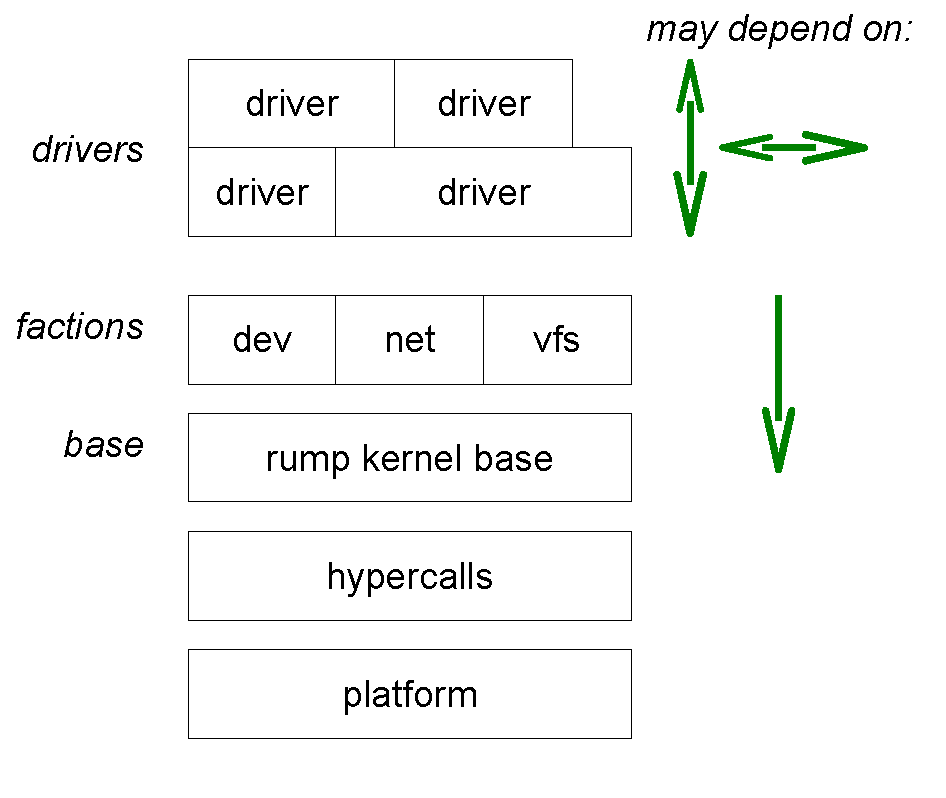
\includegraphics[height=8cm]{complevel}
\caption[Rump kernel hierarchy]{\textbf{Rump kernel hierarchy.}
The desired drivers dictate the required components.  The factions
are orthogonal and depend only on the rump kernel base.  The rump
kernel base depends purely on the hypercall layer.}
\label{fig:rumpcode}
\end{figure}

We use the term \textit{component} to describe a functional unit for a
rump kernel.  For example, a file system driver is a component.  A rump
kernel is constructed by linking together the desired set of components,
either at compile-time or at run-time.  A loose similarity exists between
kernel modules and the rump kernel approach: code is compiled once per
target architecture, and a linker is used to determine runtime features.
For a given driver to function properly, the rump kernel must be linked
with the right set of dependencies.  For example, the NFS component requires
both the file system and networking factions, but in contrast the tmpfs
component requires only the file system faction.

User interfaces are used by applications to request services from
rump kernels.  Any dependencies induced by user interfaces
are optional, as we will illustrate next.  Consider Unix-style
device driver access.  Access is most commonly done through file
system nodes in \texttt{/dev}, with the relevant user interfaces
being \textit{open} and \textit{read/write} (some exceptions to the
file system rule exist, such as Bluetooth and Ethernet interfaces
which are accessed via sockets on NetBSD).  To access a
\texttt{/dev} file system node in a rump kernel, file systems must be
supported.  Despite file system access being the standard way to access
a device, it is possible to architect an application
where the device interfaces are called directly without going
through file system code.  Doing so means skipping the permission
checks offered by file systems, calling private kernel interfaces and
generally having to write more fragile code.  Therefore, it is not
recommended as the default approach, but if need be due to resource
limitations, it is a possibility.  For example, let us assume we
have a rump kernel running a TCP/IP stack and we wish to use the BSD
Packet Filter (BPF)~\cite{mccanne:bpf}.  Access through
\texttt{/dev} is presented in Figure~\ref{fig:bpfvfs}, while direct
BPF access which does not use file system user interfaces is
presented in Figure~\ref{fig:bpfdirect}.  You will notice the first
example is similar to a regular application, while the latter is
more complex.  We will continue to refer to these examples in this
chapter when we go over other concepts related to rump kernels.

The faction divisions allow cutting down several hundred kilobytes
of memory overhead and milliseconds in startup time per instance.
While the saving per instance is not dramatic, the overall savings
are sizeable in applications such as network testing~\cite{hibler:emulab}
which require thousands of virtual instances.  For example, as we
will later measure in \chapref{evaluation}, a virtual TCP/IP stack
without file system support is 40\% smaller (400kB) than
one which contains file system support.

\subsubsection{Hosting}

To function properly, a rump kernel must access certain host resources
such as memory and the scheduler.  These resources are accessed through
the \textit{rumpuser} hypercall interface.  We will analyze and describe
this interface in detail in Section~\ref{sect:hypercall}.

Notably, as we already hinted in the introduction, the platform
requirements for a rump kernel are extremely minimal, and a rump kernel
can run virtually everywhere.  For example, there is no need to run the
rump kernel in privileged hardware mode.  Ultimately, the host has full
control and fine-grained control of what a rump kernel has access to.


\begin{figure}
{\tt \scriptsize
\begin{verbatim}
int
main(int argc, char *argv[])
{
        struct ifreq ifr;
        int fd;

        /* bootstrap rump kernel */
        rump_init();

        /* open bpf device, fd is in implicit process */
        if ((fd = rump_sys_open(_PATH_BPF, O_RDWR, 0)) == -1)
                err(1, "bpf open");

        /* create virt0 in the rump kernel the easy way and set bpf to use it */
        rump_pub_virtif_create(0);
        strlcpy(ifr.ifr_name, "virt0", sizeof(ifr.ifr_name));
        if (rump_sys_ioctl(fd, BIOCSETIF, &ifr) == -1)
                err(1, "set if");

        /* rest of the application */
        [....]
}
\end{verbatim}}
\caption[BPF access via file system]{\textbf{BPF access via the file
system.} This figure demonstrates the system call style programming interface
of a rump kernel.}
\label{fig:bpfvfs}
\end{figure}

\begin{figure}
{\tt \scriptsize
\begin{verbatim}
int rumpns_bpfopen(dev_t, int, int, struct lwp *);

int
main(int argc, char *argv[])
{
        struct ifreq ifr;
        struct lwp *mylwp;
        int fd, error;

        /* bootstrap rump kernel */
        rump_init();

        /* create an explicit rump kernel process context */
        rump_pub_lwproc_rfork(RUMP_RFCFDG);
        mylwp = rump_pub_lwproc_curlwp();

        /* schedule rump kernel CPU */
        rump_schedule();

        /* open bpf device */
        error = rumpns_bpfopen(0, FREAD|FWRITE, 0, mylwp);
        if (mylwp->l_dupfd < 0) {
                rump_unschedule();
                errx(1, "open failed");
        }

        /* need to jump through a hoop due to bpf being a "cloning" device */
        error = rumpns_fd_dupopen(mylwp->l_dupfd, &fd, 0, error);
        rump_unschedule();
        if (error)
                errx(1, "dup failed");

        /* create virt0 in the rump kernel the easy way and set bpf to use it */
        rump_pub_virtif_create(0);
        strlcpy(ifr.ifr_name, "virt0", sizeof(ifr.ifr_name));
        if (rump_sys_ioctl(fd, BIOCSETIF, &ifr) == -1)
                err(1, "set if");

        /* rest of the application */
        [....]
}
\end{verbatim}}
\caption[BPF access without a file system]{\textbf{BPF access without
a file system.}  This figure demonstrates the ability to directly
call arbitrary kernel routines from a user program.  For comparison,
it implements the same functionality as Figure~\ref{fig:bpfvfs}.
This ability is most useful for writing kernel unit tests when the calls
to the unit under test cannot be directly invoked by using the standard
system call interfaces.}
\label{fig:bpfdirect}
\end{figure}

\subsection{Rump Kernel Clients}
\label{sect:clitax}

We define a rump kernel client to be an application that requests
services from a rump kernel.  Examples of rump kernel clients are
an application that accesses the network through a TCP/IP stack
provided by a rump kernel, or an application that reads files via
a file system driver running in a rump kernel.  Likewise, a test
program that is used to test kernel code by means of running it
in a rump kernel is a rump kernel client.

The relationship between a rump kernel and a rump kernel client is
an almost direct analogy to an application process executing on an
operating system and requesting services from the host kernel.
The difference is that a rump kernel client must explicitly request
all services from the rump kernel, while a process receives some
services such as scheduling and memory protection implicitly from
the host.

As mentioned in \chapref{introduction} there are several possible relationship
types the client and rump kernel can have.  Each of them have
different implications on the client and kernel.  The possibilities
are: \textit{local}, \textit{remote} and \textit{microkernel}.
The configurations are also depicted in Figure~\ref{fig:clidiag}.
The implications of each are available in summarized form in
Table~\ref{tab:clients}.  Next, we will discuss the configurations and
explain the table.

\begin{table}[t]
\begin{tabular}{| l | l | l | l | l |}
\hline
Type & Request Policy & Access & Available Interface \\
\hline
\hline
local & client & full & all \\
\hline
remote & client & limited & system call \\
\hline
microkernel & host kernel & limited & depends on service \\
\hline
\end{tabular}
\caption[Comparison of client types]{\textbf{Comparison of client types.}
Local clients get full access to a rump kernel, but require explicit
calls in the program code.  Remote clients have standard system
call access with security control and can use unmodified binaries.
In microkernel mode, the rump kernel is run as a microkernel style system
server with requests routed by the host kernel.
}
\label{tab:clients}
\end{table}

\begin{figure}[t]
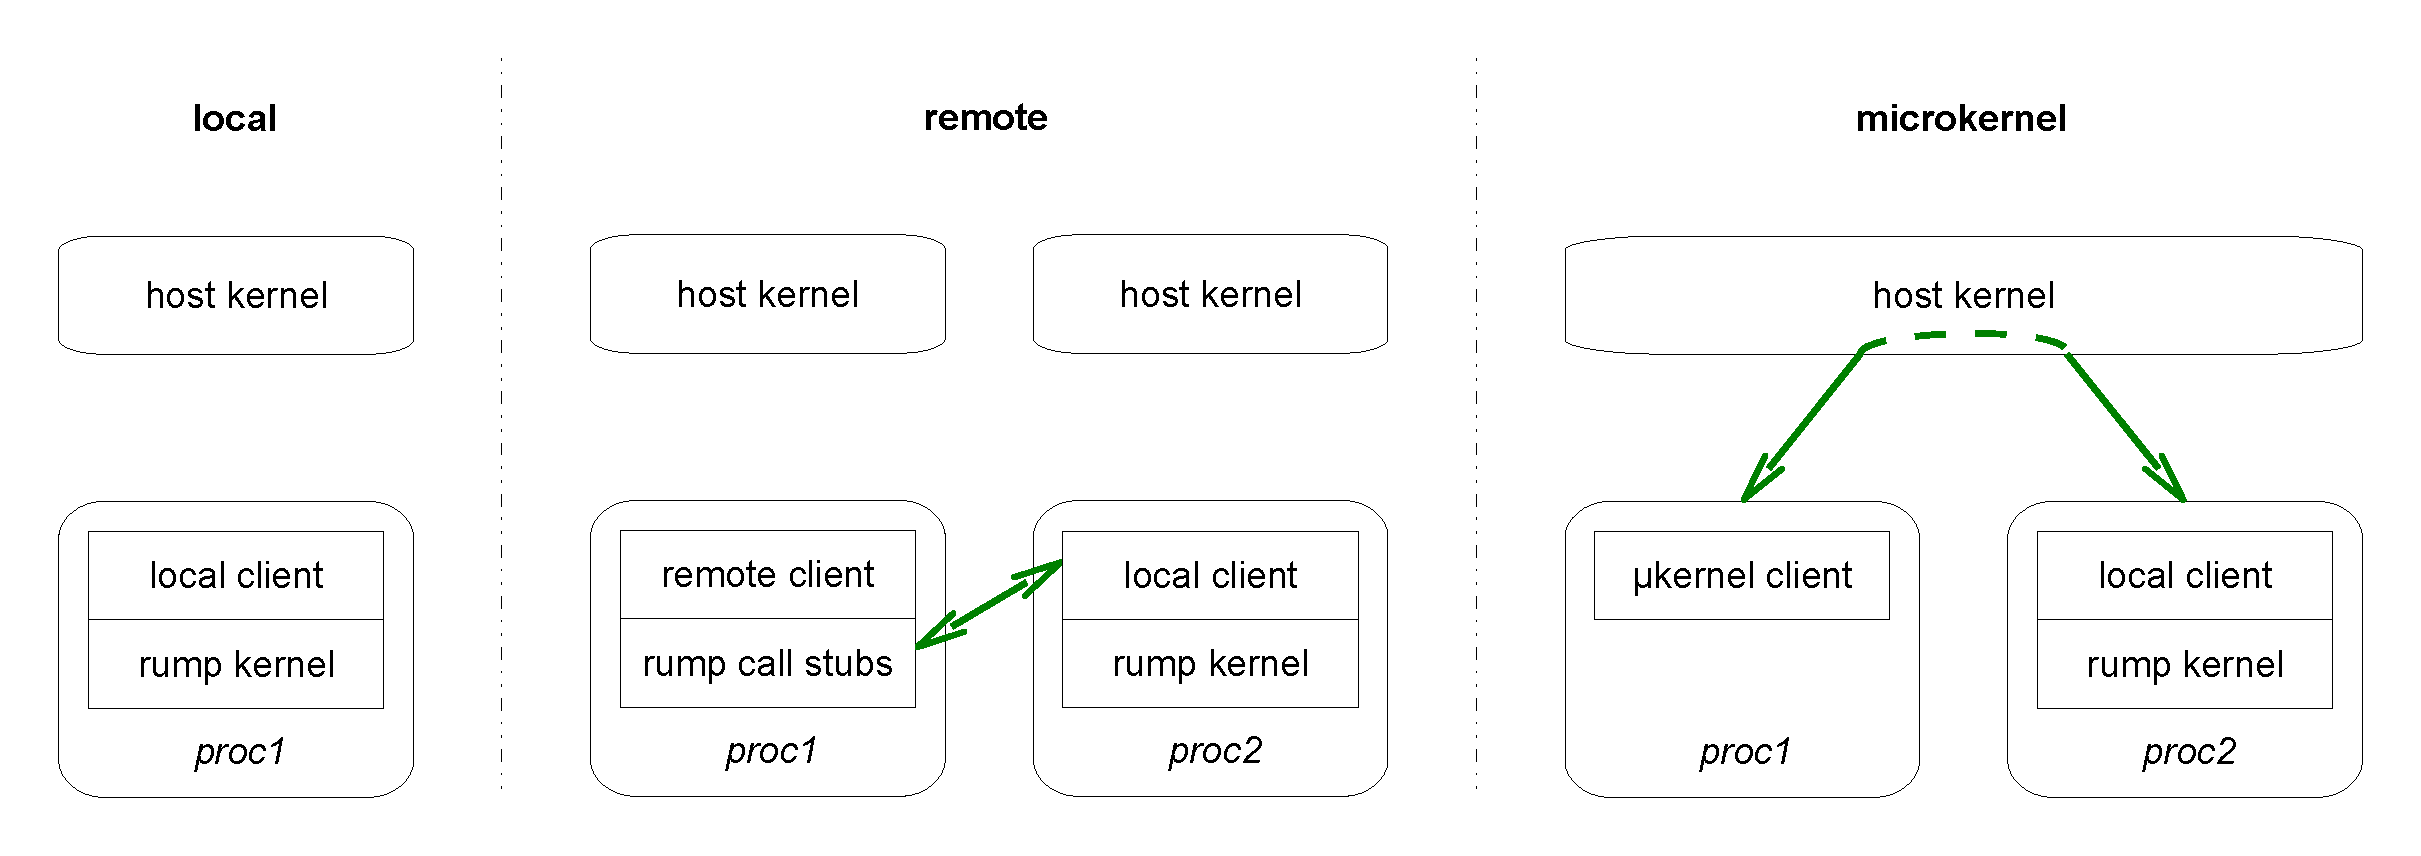
\includegraphics[width=\linewidth]{clientcomp}
\caption[Client types illustrated]{\textbf{Client types illustrated.}
For local clients the client and rump kernel reside in a single process,
while remote and microkernel clients reside in separate processes and
therefore do not have direct memory access into the rump kernel.
}
\label{fig:clidiag}
\end{figure}

\begin{itemize}
\item   \textbf{Local} clients exist in the same application process
	as the rump kernel itself.  They have full access to the
	rump kernel's address space, and make requests via function
	calls directly into the rump kernel.  Typically requests
	are done via established interfaces such as the rump kernel
	syscall interface, but there is nothing preventing the client
	from jumping to any routine inside the rump kernel.  The
	VFS-bypassing example in Figure~\ref{fig:bpfdirect} is a
	local client which manipulates the kernel directly, while
	the local client in Figure~\ref{fig:bpfvfs} uses established
	interfaces.

	The benefits of local clients include speed and compactness.
	Speed is due to a rump kernel request being essentially a
	function call.	A null rump kernel system call is twice as fast
	as a native system call.  Compactness results from the fact that
	there is only a single program and can make managing the whole
	easier.  The drawback is that the single program must configure
	the kernel to a suitable state before the application can act.
	Examples of configuration tasks include adding routing tables
	(the \texttt{route} utility) and mounting file systems (the
	\texttt{mount} utility).  Since existing configuration tools are
	built around the concept of executing different configuration
	steps as multiple invocations of the tool, adaptation of the
	configuration code may not always be simple.

	On a POSIX system, local clients do not have meaningful semantics
	for a host \texttt{fork()} call.  This lack of semantics is
	because the rump kernel state would be duplicated and could
	result in for example two kernels accessing the same file system
	or having the same IP address.

	A typical example of a local client is an application which
	uses the rump kernel as a programming library \eg to access
	a file system.

\item	\textbf{Remote} clients use a rump kernel which resides
	elsewhere, either on the local host or a remote one.  The request
	routing policy is up to the client.  The policy locus is an
	implementation decision, not a design decision, and alternative
	implementations can be considered~\cite{gardenghi:viewos} if
	it is important to have the request routing policy outside of
	the client.

	Since the client and kernel are separated, kernel side
	access control is fully enforced --- if the client and rump
	kernel are on the same host, we assume that the host enforces
	separation between the respective processes.  This separation
	means that a remote client will not be able to access resources
	except where the rump kernel lets it, and neither will it be able
	to dictate the thread and process context in which requests are
	executed.  The client not being able to access arbitrary kernel
	resources in turn means that real security models are possible,
	and that different clients may have varying levels of privileges.

	We have implemented support for remote clients which
	communicate with the server using local domain sockets or TCP
	sockets.  Using sockets is not the only option, and for example
	the \texttt{ptrace()} facility can also be used to implement
	remote clients~\cite{dike:uml,gardenghi:viewos}.

	Remote clients are not as performant as local clients due to
	IPC overhead.
	However, since multiple remote clients can run against a
	single rump kernel, they lead to more straightforward use
	of existing code and even that of unmodified binaries.

	Remote clients, unlike local clients, have meaningful semantics
	for \texttt{fork()} since both the host kernel context and
	rump kernel contexts can be correctly preserved: the host
	\texttt{fork()} duplicates only the client and not the rump
	kernel.

\item   \textbf{Microkernel} clients requests are routed by the host kernel to
	a separate server which handles the requests using a driver in a
	rump kernel.  While microkernel clients can be seen to be remote
	clients, the key difference to remote clients is that the request
	routing policy is in the host kernel instead of in the client.
	Furthermore, the interface used to access the rump kernel
	is below the system call layer.  We implemented microkernel
	callbacks for file systems (puffs~\cite{kantee:puffs})
	and \textit{character}/\textit{block} device drivers
	(pud~\cite{man4:pud}).	They use the NetBSD kernel VFS/vnode
	and \textit{cdev}/\textit{bdev} interfaces to access the rump
	kernel, respectively.
\end{itemize}

It needs to be noted that rump kernels accepting multiple different types
of clients are possible.  For example, remote clients can be used to
configure a rump kernel, while the application logic still remains in
the local client.  The ability to use multiple types of clients on a
single rump kernel makes it possible to reuse existing tools for
the configuration job and still reap the speed benefit of a local client.

Rump kernels used by remote or microkernel clients always include
a local client as part of the process the rump kernel is hosted in.
This local client is responsible for forwarding incoming requests to
the rump kernel, and sending the results back after the request has
been processed.

\subsubsection{Client and Kernel Type System Congruence}

TODO: Some mumblings motivating rumprun for Chapter 3.


\subsection{Threads and Schedulers}
\label{sect:procmodel}

Next, we will discuss the theory and concepts related to processes,
threads, CPUs, scheduling and interrupts in a rump kernel.  An
example scenario is presented after the theory in
Section~\ref{sect:lexample}.  This subject is revisited in
Section~\ref{sect:rumpentry} where we discuss it from a more concrete
perspective along with the implementation.

As stated earlier, a rump kernel uses the host's process, thread and
scheduling facilities.  To understand why we still need to discuss
this topic, let us first consider what a thread represents to an
operating system.  First, a thread represents machine execution context,
such as the program counter, other registers and the virtual memory
address space.  We call this machine context the \textit{hard context}.
It determines how machine instructions will be executed when a thread
is running on a CPU and what their effects will be.  The hard context
is determined by the platform that the thread runs on.  Second, a
thread represents all auxiliary data required by the operating system.
We call this auxiliary data the \textit{soft context}.  It comprises
for example of information determining which process a thread belongs
to, and \eg therefore what credentials and file descriptors it has.
The soft context is determined by the operating system.

To further illustrate, we go over a simplified version of what happens
in NetBSD when an application process creates a thread:

\begin{enumerate}
\item   The application calls \verb+pthread_create()+ and passes
	in the necessary parameters, including the address of the new
	thread's start routine.

\item   The pthread library does the necessary initialization, including
	stack allocation.  It creates a hard context
	by calling \verb+_lwp_makecontext()+ and passing the
	start routine's address as an argument.  The pthread library then
	invokes the \verb+_lwp_create()+ system call.

\item   The host kernel creates the kernel soft context for the
	new thread and the thread is put into the run queue.

\item	The newly created thread will be scheduled and begin execution
	at some point in the future.
\end{enumerate}

A rump kernel uses host threads for the hard context.  Local client
threads which call a rump kernel are created as described
above.  Since host thread creation does not involve the rump kernel,
a host thread does not get an associated rump kernel thread soft context
upon creation.

Nonetheless, a unique rump kernel soft context must exist for
each thread executing within the rump kernel because the code we
wish to run relies on it.  For example, code dealing with file
descriptors accesses the relevant data structure by dereferencing
\verb+curlwp->l_fd+~\footnote
{
	\texttt{curlwp} is not variable in the C language sense.
	It is a platform-specific macro which produces a pointer
	to the currently executing thread's kernel soft context.
	Furthermore, since file descriptors are a process concept
	instead of a thread concept, it would be more logical to
	access them via \texttt{curlwp->l\_proc->p\_fd}.
	The pointer is cached directly in
	the thread structure to avoid extra indirection.
}.
The soft context determines the value of \texttt{curlwp}.

We must solve the lack of a rump kernel soft context resulting from the
use of host threads.  Whenever a host thread makes a function call into
the rump kernel, an entry point wrapper must be called.  Conversely,
when the rump kernel routine returns to the client, an exit point wrapper is called.
These calls are done automatically for official interfaces, and must
be done manually in other cases --- compare Figure~\ref{fig:bpfvfs}
and Figure~\ref{fig:bpfdirect} and see that the latter includes calls
to \verb+rump_schedule()+ and \verb+rump_unschedule()+.  The wrappers
check the host's thread local storage (TLS) to see if there is a rump
kernel soft context associated with the host thread.
The soft context may either be set or not set.  We discuss
both cases in the following paragraphs.

\begin{enumerate}
\item \textbf{implicit threads}: the soft context is not set
in TLS.  A soft context will be created dynamically and is called
an \textit{implicit thread}.  Conversely, the implicit thread will be
released at the exit point.  Implicit threads are always attached to the
same rump kernel process context, so callers performing multiple calls,
\eg opening a file and reading from the resulting file descriptor,
will see expected results.  The rump kernel thread context will be
different as the previous one no longer exists when the next call
is made.  A different context does not matter, as the kernel thread
context is not exposed to userspace through any portable interfaces
--- that would not make sense for systems which implement a threading
model where userspace threads are multiplexed on top of kernel provided
threads~\cite{anderson:scheduler_activations}.

\item \textbf{bound threads}: the soft context is set in TLS.
The rump kernel soft context in the host thread's TLS can be set,
changed and disbanded using interfaces further described in the
\manpageref{rumplwproc.3}{rump\_lwproc.3}.  We call a thread with the rump
kernel soft context set a \textit{bound thread}.  All calls to the rump
kernel made from a host thread with a bound thread will be executed with
the same rump kernel soft context.
\end{enumerate}

The soft context is always set by a local client.  Microkernel and
remote clients are not able to directly influence their rump kernel thread
and process context.  Their rump kernel context is set by the local client
which receives the request and makes the local call into the rump kernel.

\subsubsection*{Discussion}

There are alternative approaches to implicit threads.  It would
be possible to require all local host threads to register with the rump
kernel before making calls.  The registration would create essentially
a bound thread.  There are two reasons why this approach was not chosen.
First, it increases the inconvenience factor for casual users, as they
now need a separate call per host thread.  Second, some mechanism
like implicit threads must be implemented anyway: allocating a rump
kernel thread context requires a rump kernel context for example to be
able to allocate memory for the data structures.  Our implicit thread
implementation doubles as a bootstrap context.

Implicit contexts are created dynamically because because any
preconfigured reasonable amount of contexts risks application deadlock.
For example, $n$ implicit threads can be waiting inside the rump kernel
for an event which is supposed to be delivered by the $n+1$'th implicit
thread, but only $n$ implicit threads were precreated.  Creating an
amount which will never be reached (\eg 10,000) may avoid deadlock,
but is wasteful.  Additionally, we assume all users aiming for high
performance will use bound threads.

\subsubsection{Kernel threads}

Up until now, we have discussed the rump kernel context of threads which
are created by the client, typically by calling \verb+pthread_create()+.
In addition, \textit{kernel threads} exist.  The creation of a kernel
thread is initiated by the kernel and the entry point lies within the
kernel.  Therefore, a kernel thread always executes within the kernel
except when it makes a hypercall.  Kernel threads are associated
with process~0 (\texttt{struct~proc0}).  An example of a kernel thread
is the \textit{workqueue worker} thread, which the workqueue kernel
subsystem uses to schedule and execute asynchronous work units.

On a regular system, both an application process thread and a kernel
thread have their hard context created by the kernel.  As we mentioned
before, a rump kernel cannot create a hard context.  Therefore, whenever
kernel thread creation is requested, the rump kernel creates the soft
context and uses a hypercall to request the hard context from the host.
The entry point given to the hypercall is a bouncer routine inside
the rump kernel.  The bouncer first associates the kernel thread's
soft context with the newly created host thread and then proceeds to
call the thread's actual entry point.

\subsubsection{A CPU for a Thread}
\label{sect:cpusched}

First, let us use broad terms to describe how scheduling works in regular
virtualized setup.  The hypervisor has an idle CPU it wants to schedule
work onto and it schedules a guest system.  While the guest system is
running, the guest system decides which guest threads to run and when
to run them using the guest system's scheduler.  This means that there
are two layers of schedulers involved in scheduling a guest thread.

We also point out that a guest CPU can be a purely virtual entity, \eg
the guest may support multiplexing a number of virtual CPUs on top of
one host CPU.  Similarly, the rump kernel may be configured to provide
any number of CPUs that the guest OS supports regardless of the number of
CPUs present on the host.  The default for a rump kernel is to provide the
same number of virtual CPUs as the number of physical CPUs on the host.
Then, a rump kernel can fully utilize all the host's CPUs, but will not
waste resources on virtual CPUs where the host cannot schedule threads
for them in parallel.

As a second primer for the coming discussion, we will review
CPU-local algorithms.  CPU-local algorithms are used avoid slow
cross-CPU locking and hardware cache invalidation.  Consider a
pool-style resource allocator (\eg memory): accessing a global pool
is avoided as far as possible because of the aforementioned reasons
of locking and cache.  Instead, a CPU-local allocation cache for
the pools is kept.  Since the local cache is tied to the CPU, and since
there can be only one thread executing on one CPU at a time, there is
no need for locking other than disabling thread preemption in the kernel
while the local cache is being accessed.  Figure~\ref{fig:curcpu}
gives an illustrative example.

The host thread doubles as the guest thread in a rump kernel and the host
schedules guest threads.  The guest CPU is left out of the relationship.
The one-to-one relationship between the guest CPU and the guest thread
must exist because CPU-local algorithms rely on that invariant.  If we
remove the restriction of each rump kernel CPU running at most one thread
at a time, code written against CPU-local algorithms will cause data
structure corruption and fail.  Therefore, it is necessary to uphold
the invariant that a CPU has at most one thread executing on it at a time.

\begin{figure}[t]
{\tt \scriptsize
\begin{alltt}
void *
pool_cache_get_paddr(pool_cache_t pc)
\{
    pool_cache_cpu_t *cc;

    cc = pc->pc_cpus[\textcolor{blue}{curcpu()}->ci_index];
    pcg = cc->cc_current;
    if (__predict_true(pcg->pcg_avail > 0)) \{
            /* fastpath */
            object = pcg->pcg_objects[--pcg->pcg_avail].pcgo_va;
            return object;
    \} else \{
            return pool_cache_get_slow();
    \}
\}
\end{alltt}}
\caption[Use of \texttt{curcpu()} in the pool allocator]
{\textbf{Use of \texttt{curcpu()} in the pool allocator}
simplified as pseudocode from \texttt{sys/kern/subr\_pool.c}.
An array of CPU-local caches is indexed by the current CPU's number to
obtain a pointer to the CPU-local data structure.  Lockless allocation
from this cache is attempted before reaching into the global pool.
}
\label{fig:curcpu}
\end{figure}

Since selection of the guest thread is handled by the host, we select the
guest CPU instead.  The rump kernel virtual CPU is assigned for the thread
that was selected by the host, or more precisely that thread's rump kernel
soft context.  Simplified, scheduling in a rump kernel can be considered
picking a CPU data structure off of a freelist when a thread enters the
rump kernel and returning the CPU to the freelist once a thread exits
the rump kernel.  A performant implementation is more delicate due to
multiprocessor efficiency concerns.  One is discussed in more detail along
with the rest of the implementation in Section~\ref{sect:cpuschedimpl}.

Scheduling a CPU and releasing it are handled at the rump kernel
entrypoint and exitpoint, respectively.  The BPF example with VFS
(Figure~\ref{fig:bpfvfs}) relies on rump kernel interfaces handling
scheduling automatically for the clients.  The BPF example which calls
kernel interfaces directly (Figure~\ref{fig:bpfdirect}) schedules a CPU
before it calls a routine inside the rump kernel.

\subsubsection{Interrupts and Preemption}
\label{sect:preempt}

An interrupt is an asynchronously occurring event which preempts
the current thread and proceeds to execute a compact handler for
the event before returning control back to the original thread.
The interrupt mechanism allows the OS to quickly acknowledge especially
hardware events and schedule the required actions for a suitable time
(which may be immediately).  Taking an interrupt is tied to the concept
of being able to temporarily replace the currently executing thread with
the interrupt handler.  Kernel thread preemption is a related concept
in that code currently executing in the kernel can be removed from
the CPU and a higher priority thread selected instead.

The rump kernel uses a cooperative scheduling model where the
currently executing thread runs to completion.  There is no virtual CPU
preemption, neither by interrupts nor by the scheduler.  A thread holds
on to the rump kernel virtual CPU until it either makes a blocking
hypercall or returns from the request handler.  A host thread
executing inside the rump kernel may be preempted by the host.  Preemption
will leave the virtual CPU busy until the host reschedules the preempted
thread and the thread runs to completion in the rump kernel.

What would be delivered by a preempting interrupt in the monolithic
kernel is always delivered via a schedulable thread in a rump kernel.
In the event that later use cases present a strong desire for fast
interrupt delivery and preemption, the author's suggestion is to
create dedicated virtual rump CPUs for interrupts and real-time
threads and map them to high-priority host threads.  Doing so avoids
interaction with the host threads via signal handlers (or
similar mechanisms on other non-POSIX host architectures).  It is
also in compliance with the paradigm that the host handles all
scheduling in a rump kernel.

\subsubsection{An Example}
\label{sect:lexample}

We present an example to clarify the content of this subsection.
Let us assume two host threads, A and B, which both act as local clients.
The host schedules thread A first.  It makes a call into the rump kernel
requesting a bound thread.  First, the soft context for an implicit thread
is created and a CPU is scheduled.  The implicit thread soft context is
used to create the soft context of the bound thread.  The bound thread
soft context is assigned to thread A and the call returns after free'ing
the implicit thread and releasing the CPU.  Now, thread A calls the
rump kernel to access a driver.  Since it has a bound thread context,
only CPU scheduling is done.  Thread A is running in the rump kernel and
it locks mutex M.  Now, the host scheduler decides to schedule thread
B on the host CPU instead.  There are two possible scenarios:

\begin{enumerate}
\item The rump kernel is a uniprocessor kernel and thread B will be blocked.
This is because thread A is still scheduled onto the only rump kernel
CPU.  Since there is no preemption for the rump kernel context, B will
be blocked until A runs and releases the rump kernel CPU.  Notably,
it makes no difference if thread B is an interrupt thread or not ---
the CPU will not be available until thread A releases it.

\item The rump kernel is a multiprocessor kernel and there is a
chance that other rump kernel CPUs may be available for thread B to be
scheduled on.  In this case B can run.
\end{enumerate}

We assume that B can run immediately.  Thread B uses implicit threads, and
therefore upon entering the rump kernel an implicit thread soft context
gets created and assigned to thread B, along with a rump kernel CPU.

After having received a rump kernel CPU and thread context, thread B
wants to lock mutex M.  M is held, and thread B will have to block and
await M's release.  Thread B will release the rump kernel CPU and sleep
until A unlocks the mutex.  After the mutex
is unlocked, the host marks thread B as runnable and after B wakes up,
it will attempt to schedule a rump kernel CPU and after that attempt
to lock mutex M and continue execution.  When B is done with the rump
kernel call, it will return back to the application.  Before doing so,
the CPU will be released and the implicit thread context will be free'd.

Note that for thread A and thread B to run in \textit{parallel}, both
the host and the rump kernel must have multiprocessor capability.
If the host is uniprocessor but the rump kernel is configured with
multiple virtual CPUs, the threads can execute inside the rump
kernel \textit{concurrently}.  In case the rump kernel is configured
with only one CPU, the threads will execute within the rump kernel
\textit{sequentially} irrespective of if the host has one or more CPUs
available for the rump kernel.

\subsection{Virtual Memory}
\label{sect:vmconcept}

Virtual memory address space management in a rump kernel is relegated
to the host because support in a rump kernel would
not add value in terms of the intended use cases.  The only case
where full virtual memory support would be helpful would be for
testing the virtual memory subsystem.  Emulating page faults and
memory protection in a usermode OS exhibits over tenfold performance
penalty and can be significant in other, though not all,
hypervisors~\cite{barham:xen}.  Therefore, supporting a corner use
case was not seen worth the performance penalty in other use cases.

The implication of a rump kernel not implementing full memory
protection is that it does not support accessing resources via page
faults.  There is no support in a rump kernel for memory mapping a file
to a client.  Supporting page faults \textit{inside} a rump kernel would
not work for remote clients anyway, since the page faults need to be
trapped on the client machine.

\begin{figure}[t]
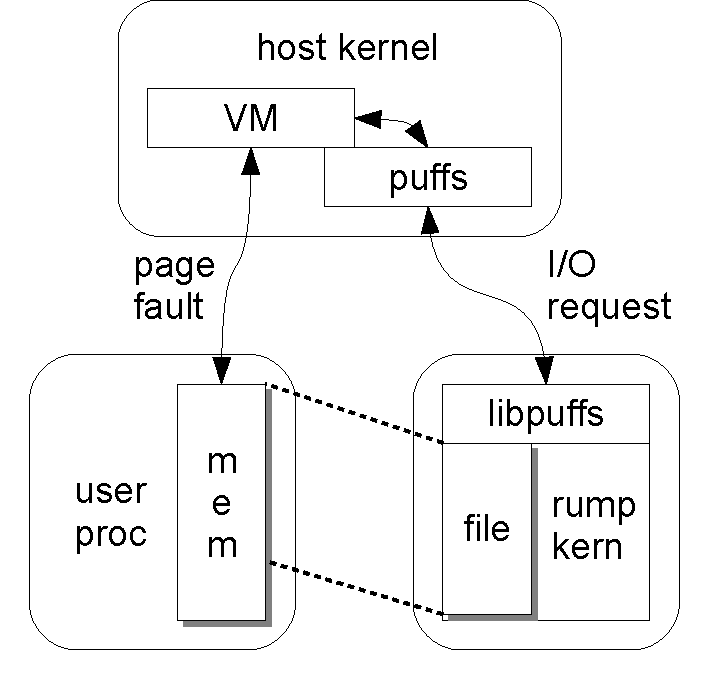
\includegraphics[height=6cm]{puffsfault}
\caption[Providing memory mapping support on top of a rump kernel]
{\textbf{Providing memory mapping support on top of a rump kernel}.
The file is mapped into the client's address space by the host kernel.
When non-resident pages in the mapped range are accessed by the client,
a page fault is generated and the rump kernel is invoked via
the host kernel's file system code to supply the desired data.}
\label{fig:puffsmmap}
\end{figure}

However, it is possible to provide memory
mapping \textit{on top} of rump kernels.  In fact, when running
file systems as microkernel servers, the puffs~\cite{kantee:puffs}
userspace file system framework and the host kernel provide memory
mapping for the microkernel client.  The page fault is resolved
in the host kernel, and the I/O request for paging in the necessary data
sent to the rump kernel.  After the rump kernel has satisfied the request
and responded via puffs, the host kernel unblocks the process that caused
the page fault (Figure~\ref{fig:puffsmmap}).  If a desirable use case is
found, distributed shared memory~\cite{minnich:mether} can be investigated
for memory mapping support in remote clients.

Another implication of the lack of memory protection is that a
local client can freely access the memory in a rump kernel.
Consider the BPF example which accesses the kernel directly
(Figure~\ref{fig:bpfdirect}).  Not only does the local client call
kernel routines, it also examines the contents of a kernel data
structure.

\subsection{Distributed Services with Remote Clients}
\label{sect:distributed}

As mentioned in our client taxonomy in Section~\ref{sect:clitax},
remote clients use services from a rump kernel hosted either on
the same host in another process or on a remote host.  We describe
the general concept here and provide implementation details later
in Section~\ref{sect:sysproxyimpl}.

It is known to be possible to build a Unix system call emulation
library on top of a distributed system~\cite{mullender:amoeba}.
We go further: while we provide the Unix interface to applications,
we also use existing Unix kernel code at the server side.

Running a client and the rump kernel on separate hosts is possible
because on a fundamental level Unix already works like a
distributed system: the kernel and user processes live in different
address spaces and information is explicitly moved across this boundary
by the kernel.  Copying data across the boundary simplifies the kernel,
since data handled by the kernel can always be assumed to be resident and
non-changing.  Explicit copy requests in the kernel code make it possible
to support remote clients by implementing only a request transport layer.
System calls become RPC requests from the client to the kernel
and routines which copy data between arbitrary address spaces become
RPC requests from the kernel to the client.

When a remote client connects to a rump kernel, it gets assigned a rump
kernel process context with appropriate credentials.  After the handshake
is complete, the remote client can issue service requests via the standard
system call interface.  First, the client calls a local stub routine,
which marshalls the request.  The stub then sends the request to the
server and blocks the caller.  After the rump kernel server has processed
the request and responded, the response is decoded and the client is
unblocked.  When the connection between a rump kernel and a remote client
is severed, the rump kernel treats the client process as terminated.

The straightforward use of existing data structures has its limitations:
the system the client is hosted on must share the same ABI with the
system hosting the rump kernel.  Extending support for systems which are
not ABI-compatible is beyond the scope of our work.  However, working
remote client support shows that it is possible to build distributed
systems out of a Unix codebase without the need for a new design and
codebase such as Plan~9~\cite{pike:plan9}.

\subsection{Summary}

A rump kernel is a partial virtualization of an operating system kernel
with the virtualization target being the drivers.  To be as lightweight
as possible, a rump kernel relies on two features: relegating support
functionality to the host where possible and an anykernel codebase
where different units of the kernel (\eg networking and file systems)
are disjoint enough to be usable in configurations where all parties
are not present.

Rump kernels support three types of clients: local, microkernel
and remote.  Each client type has its unique properties and varies for
example in access rights to a rump kernel, the mechanism for making
requests, and performance characteristics.  Remote clients are able to
access a rump kernel over the Internet.

For drivers to function, a rump kernel must possess runtime context
information.  This information consists of the process/thread
context and a unique rump kernel CPU that each thread is associated
with.  A rump kernel does not assume virtual memory, and does not
provide support for page faults or memory protection.  Virtual
memory protection and page faults, where necessary, are always
left to be performed by the host of the rump kernel client.
